\begin{table}[]
    \centering
    \begin{tabular}{ccc}
    \toprule
    x (cm) & Temperature (\si{\celsius}) & Temperature (\si{\celsius})\\
    & Non-mixing & Mixing \\
    \midrule
    0 & 27.9 & 28.2\\
    1.5 & 27.9 & 28.3\\
    3.0 & 27.9 & 28.4\\
    \bottomrule
    \end{tabular}
    \caption{Radial temperature variation without insulation under mixing versus non-mixing conditions}
    \label{tb:RadialTempVariation}
\end{table}
\begin{table}
    \centering
    \begin{tabular}{ccc}
    \toprule
    y (cm) & Temperature(\si{\celsius}) & Temperature(\si{\celsius})\\
    & Non-mixing & Mixing \\
    \midrule
    1.5 & 29.4 & 28.7 \\
    4.5 & 28.9 & 28.7 \\
    7.5 & 26.7 & 28.6 \\
    \bottomrule
    \end{tabular}
    \caption{Vertical temperature variation without insulation under mixing versus non-mixing conditions}
    \label{tb:VerticalTempVariation}
\end{table}

From Tables \ref{tb:RadialTempVariation},\ref{tb:VerticalTempVariation}, the means of radial and vertical temperature measurements under mixing condition, 28.3\si{\celsius} and 28.7 \si{\celsius}, respectively, are higher than the ones under non-mixing condition, 27.9\si{\celsius} and 28.3\si{\celsius}. Therefore, mixing helps to better distribute the heat and achieve a higher liquid temperature. This is further proved by the vertical temperature standard deviation of 0.06 under mixing, a much smaller value than the 1.4 for nonmixing. 

\begin{figure}[h] %Mixing, insulated vs non insulated
    \caption*{The impacts of insulation on temperature change under mixing condition}
   \begin{minipage}{0.45\textwidth}
       \centering
   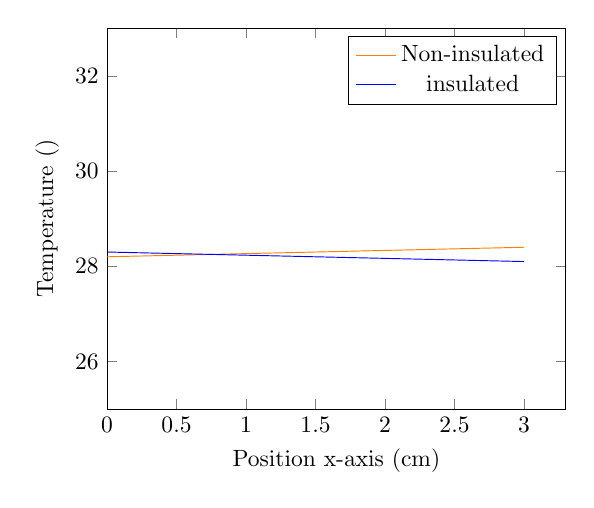
\begin{tikzpicture}[scale=0.85]
       \begin{axis}[
           xlabel= Position x-axis (cm), ylabel=Temperature (\si{\celsius}), xmin=0, ymin=25, ymax=33
       ]
       \addplot[orange] table[]{
           0   28.2
           1.5 28.3
           3.0 28.4
       };
       \addplot[blue] table[]{
           0   28.3
           1.5 28.2
           3.0 28.1
       };
       \legend{Non-insulated, insulated}
       \end{axis}
       \end{tikzpicture}
   \end{minipage}
   \begin{minipage}{0.45\textwidth}
       \centering
       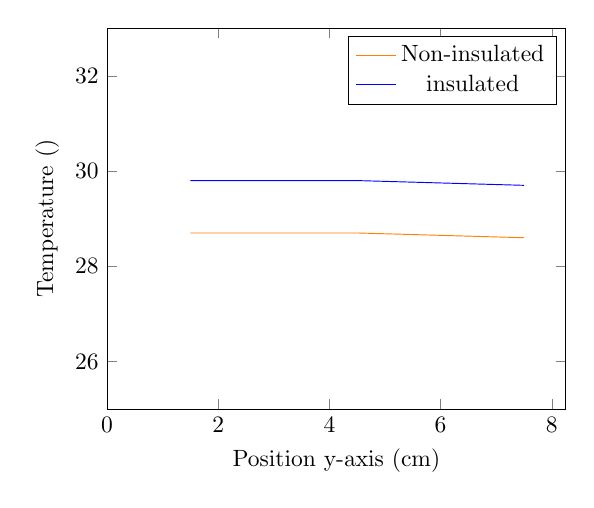
\begin{tikzpicture}[scale=0.85]
           \begin{axis}[
               xlabel= Position y-axis (cm), ylabel=Temperature (\si{\celsius}), xmin=0, ymin=25, ymax=33
           ]
               \addplot[orange] table[]{
                   1.5 28.7
                   4.5 28.7
                   7.5 28.6
               };
               \addplot[blue] table[]{
                   1.5 29.8
                   4.5 29.8
                   7.5 29.7
               };
               \legend{Non-insulated, insulated}
           \end{axis}
       \end{tikzpicture}
   \end{minipage}
   \caption{Radial(left) and vertical(right) temperature variation with and without insulation under mixing condition}
	\label{fig:Mixing-InsulationComparison}
\end{figure}

From Figure \ref{fig:Mixing-InsulationComparison}, insulation does not have a distinct impact on radial temperature variation; however, it does on vertical temperature variation. The mean of vertical temperature measurement with insulation is 29.8\si{\celsius}, approximately 4\% higher than 28.7\si{\celsius} from measurements without insulation.  

\begin{figure}[h]
    \centering
   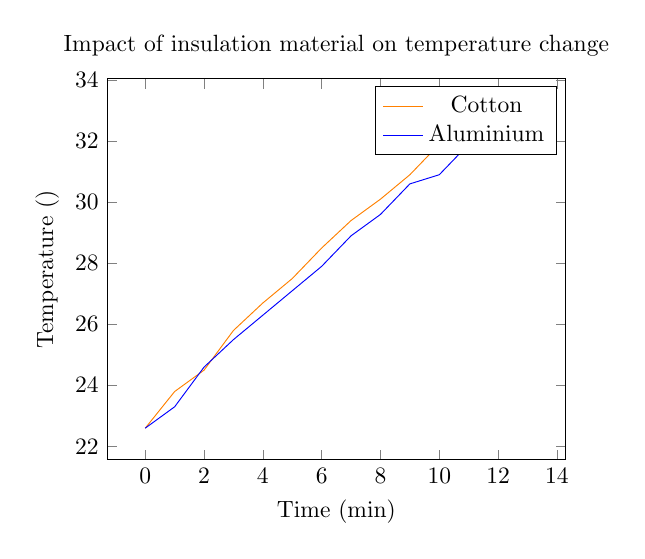
\begin{tikzpicture}[scale=0.85]
       \begin{axis}[
           title={Impact of insulation material on temperature change},xlabel= Time (min), ylabel=Temperature (\si{\celsius})
       ]
       \addplot[orange] table[]{
            0	22.6
            1	23.8
            2	24.5
            3	25.8
            4	26.7
            5	27.5
            6	28.5
            7	29.4
            8	30.1
            9	30.9
            10	31.9
            11	33
       };
       \addplot[blue] table[]{
            0	22.6
            1	23.3
            2	24.6
            3	25.5
            4	26.3
            5	27.1
            6	27.9
            7	28.9
            8	29.6
            9	30.6
            10	30.9
            11	31.9
            12	32.5
            13	33
       };
       \legend{Cotton, Aluminium}
       \end{axis}
       \end{tikzpicture}
    \caption{Temperature change over time with cotton versus aluminum foil under mixing condition}
    \label{gr:InsulationMethods}
\end{figure}

From Figure \ref{gr:InsulationMethods}, when cotton wrap is used as an insulator, 33\si{\celsius} was achieved within 11 minutes whereas when aluminum foil was used the same temperature was achieved within 13 minutes, indicating cotton to be a better choice of insulator.

\begin{figure}[h!] %Optimal thickness of insulation
\caption*{Impact of cotton layer thickness on temperature change}
   \begin{minipage}{0.45\textwidth}
       \centering
   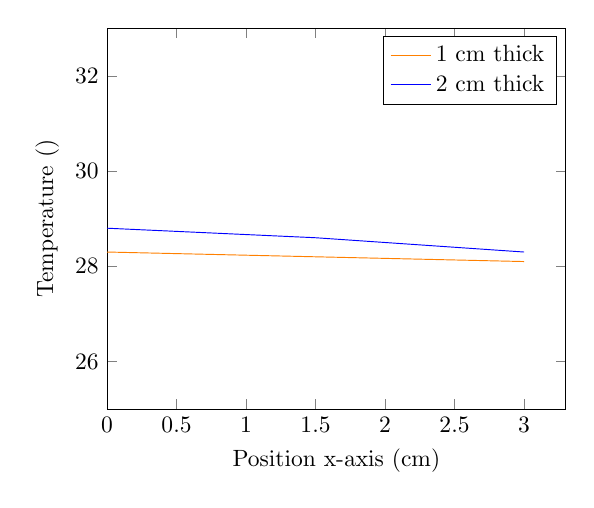
\begin{tikzpicture}[scale=0.85]
       \begin{axis}[
           xlabel= Position x-axis (cm), ylabel=Temperature (\si{\celsius}), xmin=0, ymin=25, ymax=33
       ]
       \addplot[orange] table[]{
           0   28.3
           1.5 28.2
           3.0 28.1
       };
       \addplot[blue] table[]{
           0   28.8
           1.5 28.6
           3.0 28.3
       };
       \legend{1 cm thick, 2 cm thick}
       \end{axis}
       \end{tikzpicture}
   \end{minipage}
   \begin{minipage}{0.45\textwidth}
       \centering
       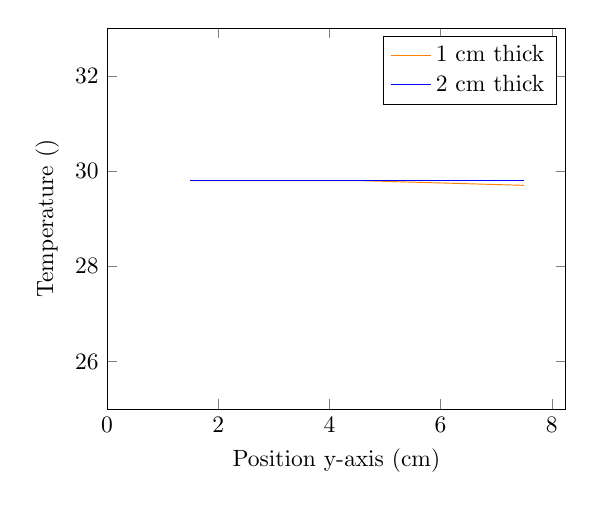
\begin{tikzpicture}[scale=0.85]
           \begin{axis}[
               xlabel= Position y-axis (cm), ylabel=Temperature (\si{\celsius}), xmin=0, ymin=25, ymax=33
           ]
               \addplot[orange] table[]{
                   1.5 29.8
                   4.5 29.8
                   7.5 29.7
               };
               \addplot[blue] table[]{
                   1.5 29.8
                   4.5 29.8
                   7.5 29.8
               };
               \legend{1 cm thick, 2 cm thick}
           \end{axis}
       \end{tikzpicture}
   \end{minipage}
   \caption{Radial(left) and vertical(right) temperature variation with 1cm-thick cotton layer versus 2cm-thick cotton layer}
	\label{gr:ThicknessComparison}
\end{figure}
From Figure \ref{gr:ThicknessComparison}, with 2cm-thick cotton layer, the means of temperature are higher than those with 1cm-thick cotton layer both radially and vertically, suggesting 2 cm to be the thickness of cotton to be used in the 24-hour run.

\begin{figure}[h!] %With and without lid, 2cm insulation
\caption*{Impact of aluminium lid on temperature change}
   \begin{minipage}{0.45\textwidth}
       \centering
   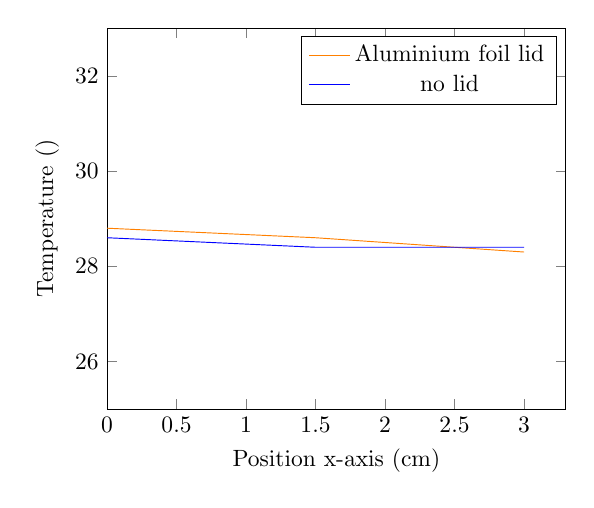
\begin{tikzpicture}[scale=0.85]
       \begin{axis}[
           xlabel= Position x-axis (cm), ylabel=Temperature (\si{\celsius}), xmin=0, ymin=25, ymax=33
       ]
       \addplot[orange] table[]{
           0   28.8
           1.5 28.6
           3.0 28.3
       };
       \addplot[blue] table[]{
           0   28.6
           1.5 28.4
           3.0 28.4
       };
       \legend{Aluminium foil lid, no lid}
       \end{axis}
       \end{tikzpicture}
   \end{minipage}
   \begin{minipage}{0.45\textwidth}
       \centering
       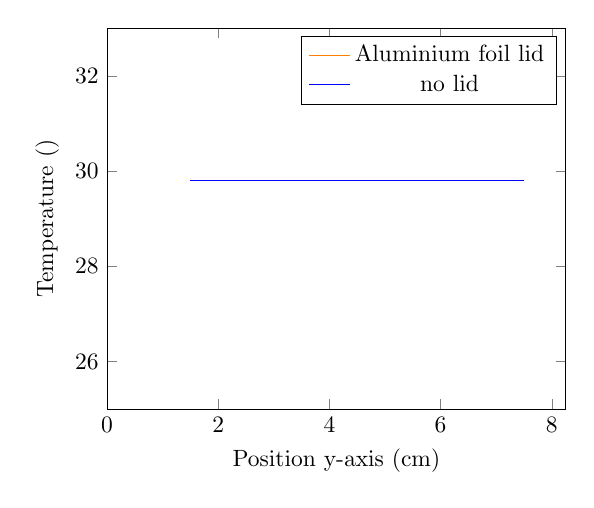
\begin{tikzpicture}[scale=0.85]
           \begin{axis}[
               xlabel= Position y-axis (cm), ylabel=Temperature (\si{\celsius}), xmin=0, ymin=25, ymax=33
           ]
               \addplot[orange] table[]{
                   1.5 29.8
                   4.5 29.8
                   7.5 29.8
               };
               \addplot[blue] table[]{
                   1.5 29.8
                   4.5 29.8
                   7.5 29.8
               };
               \legend{Aluminium foil lid, no lid}
           \end{axis}
       \end{tikzpicture}
   \end{minipage}
   \caption{Radial(left) and vertical(right) temperature variation with 2cm-thick cotton layer and Aluminum lid versus without lid}
	\label{gr:LidComparison}
\end{figure}

From Figure \ref{gr:LidComparison} Aluminum lid does not have apparent influence on temperature maintenance; therefore, will not be used in the final set up. Thus, our prototype uses 2cm-thick cotton layer as insulator under mixing condition with hot plate set to 35\si{\celsius}.

\subsubsection{Calculations}
Temperature recorded ranged from 28 to 30 \si{\celsius}, therefore we take an average between the values for \SI{27}{\celsius} and \SI{32}{\celsius} \cite{doi:10.1063/1.555963}. Furthermore, the cup is a truncated cone, and therefore its area can be calculated as:
\begin{equation}
    \begin{split}
        A &= (5+3)\pi \sqrt{{(5-3)}^2} + 8^2 = \SI{0.0207}{\meter} \\
        k_w &= \SI{0.614}{\watt\per\meter\per\celsius}
    \end{split}
\end{equation}

Utilising Fourier's law of heat, equation (\ref{eq:HeatFlux}), we calculate heat flux in each direction and summarise in Table \ref{tb:HeatFlux}.

\begin{table}[h!]
    \begin{tabular}{c c c}
        \toprule
         & Heat flux (x-direction) $\si{\watt} \cdot 10^{-4}$ & Heat flux (y-direction) $(\si{\watt}) \cdot 10^{-4}$ \\
        \midrule
        1 cm thick cotton	&	8.48	&	2.12	\\
        Without insulation	&	-8.48	&	2.12	\\
        \bottomrule
    \end{tabular}
    \caption{Heat flux under different conditions}
    \label{tb:HeatFlux}
\end{table}

From Table \ref{tb:HeatFlux}, The difference between heat induction with and without insulation is not apparent here, with a magnitude of $10^{-8}$, but can be huge in industrial scale. One consideration for scaling this prototype is to use a jacketed bioreactor and temperature control system.  

\subsubsection{24 h run prototype results}
\begin{figure}[h!]
    \centering
    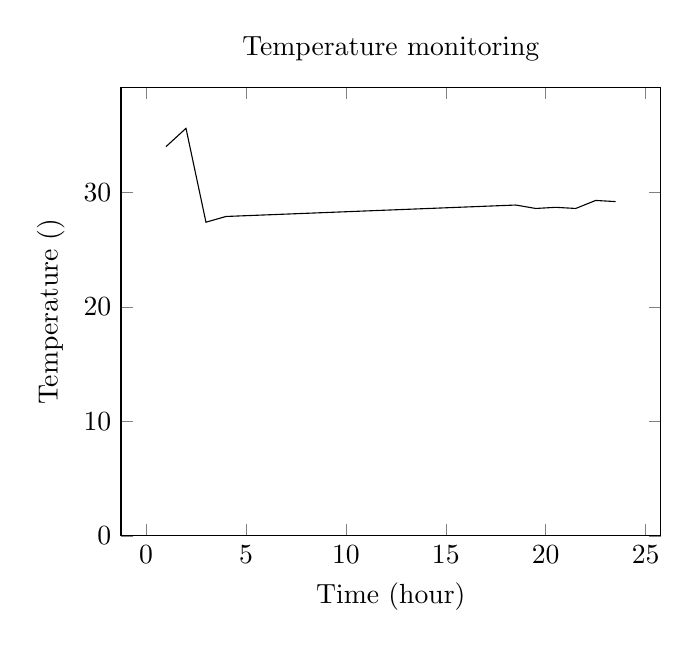
\begin{tikzpicture}[]
        \begin{axis}[title={Temperature monitoring}, ylabel=Temperature (\si{\celsius}) , xlabel=Time (hour), legend pos = south east, ymin=0]
            \addplot[] table{
            1	34.0
            2	35.6
            3	27.4
            4	27.9
            18.5	28.9
            19.5	28.6
            20.5	28.7
            21.5	28.6
            22.5	29.3
            23.5	29.2
            };
        \end{axis}
    \end{tikzpicture}
    \caption{Temperature variation over 24 hours}
\end{figure}

The prototype was set up as described in section 4.3, and temperature of the bioreactor was taken at regular interval. A graph of the recorded temperature was plotted. From Figure.2.16, temperature raised quickly at the beginning, reaching 35.6\si{\celsius} in two hours. This temperature was unexpected, so we decided to lower the hot plate temperature to 30\si{\celsius}. Temperature dropped to 27.4\si{\celsius} consequently, and maintained between 28.5-29.5\si{\celsius} after 5 hours as desired.  

\subsubsection{Fouling prevention techniques}
Fouling is the accumulation of unwanted materials such as scale, biomass and insoluble salts, on the internal or external surfaces of reactors. Fouling significantly impacts the efficiency of the reactors, reducing the flow of heat. One technique to prevent fouling would be to use anti-fouling coatings such as Notak\texttrademark\ and Dursan\textsuperscript \textregistered\  which can be applied to the surface of the reactor. The anti-fouling coating is introduced as a gas and penetrates the surface of the reactor to create a micro thin coating on the surface, which acts as a barrier. Another method to prevent fouling is through the material selection when designing the equipment. Using materials that do not easily corrode or with a low-fouling surface such as smooth surfaces or has low surface energy will reduce the chance of fouling from occurring \cite{Ibrahim12}. If fouling has already occurred steam cleaning would assist in clearing the unwanted materials on the surfaces of the equipment, however this is not always effective and impacts the process productivity \cite{KillcrossMartin2012CPT}.